\documentclass[12pt]{article}
\usepackage[utf8]{inputenc}
\usepackage[english]{babel}
\usepackage{amsmath}
\usepackage{bm}
\usepackage{listings}
\usepackage{minted}
\usepackage{graphicx}
\usepackage{subfig}

\graphicspath{./images/}
\setlength\parindent{0pt} % Removes all indentation from paragraphs
\newcommand{\uvec}[1]{\boldsymbol{\hat{\textbf{#1}}}}
\title{ECE421 - Winter 2021 \\ Logistic Regression}
\author{Shayshu Nahata-Ragubance}
\date{\today}
\begin{document}
\maketitle

\section{Objective}
Implement a simple logistic regression classifier using Numpy and
train the model by applying (Stochastic) Gradient Descent algorithm. Implement
the same model, this time in TensorFlow and use Stochastic Gradient Descent and ADAM.

\section{Logistic Regression with Numpy}
Logistic regression is one the most widely used linear classification models in machine learning. In
logistic regression, we model the probability of a sample x belonging to the positive class as

\begin{center}
  $\hat{y}(\mathbf{x}) = \theta (\mathbf{w}^T\mathbf{x} + b),$
\end{center}

where $z = \mathbf{w}^T\mathbf{x} + b$  also called logit, is basically the linear transformation of input vector $\mathbf{x}$ using
weight vector $\mathbf{w}$ and bias scalar $b$, and $\theta (z) = 1/(1 + \exp(-z))$ is the sigmoid or logistic function.
The sigmoid function “squashes” the real-valued logits to fall between zero and one.

The cross-entropy loss LCE and the regularization term Lw will form the total loss function as:
\begin{center}

  $L = L_{ce} + L_{w}$

  $L = \frac{1}{N} \sum_{n = 1}^{d} [-y_n log( \hat{y}(\mathbf{x_n})) -  (1-y_n)log(1- \hat{y}(\mathbf{x_n}))]  +  \frac{\lambda}{2}||\mathbf{w}||_2^2$
  , where $\hat{y} = \theta(\mathbf{w}^T\mathbf{x} + b)$
\end{center}

\subsection{Loss Function and Gradient}
Analytic expressions of loss shown above.
Analytic expression of gradient:
\begin{center}
  $\nabla L = \frac{1}{N} \sum_{n=1}^{N} -y_nx_n\theta (-y_nw^Tx_n) \hspace{1mm}+ \hspace{1mm} \lambda \vec{w} $

  $\nabla L = \frac{1}{N}\boldsymbol{X}^Tp \hspace{2mm} + \lambda \vec{w}\hspace{2mm}, where \hspace{2mm} p = \begin{bmatrix}
      \theta(\vec{w^T}\vec{x_1} + \hspace{1mm}b) \hspace{1mm}-\hspace{1mm}y_1 \\
      \vdots                                                                  \\
      \theta(\vec{w^T}\vec{x_N} + \hspace{2mm}b) \hspace{2mm}-\hspace{2mm}y_N \\
    \end{bmatrix} \hspace{2mm} and \hspace{2mm} \nabla = \begin{bmatrix}
      \frac{\partial}{\partial{w_1}} \\
      \frac{\partial}{\partial{w_2}} \\
      \vdots                         \\
      \frac{\partial}{\partial{w_d}} \\
    \end{bmatrix}$

  $\nabla L = \frac{1}{N}p \hspace{2mm}, where \hspace{2mm} p = \begin{bmatrix}
      \theta(\vec{w^T}\vec{x_1} + \hspace{1mm}b) \hspace{1mm}-\hspace{1mm}y_1 \\
      \vdots                                                                  \\
      \theta(\vec{w^T}\vec{x_N} + \hspace{2mm}b) \hspace{2mm}-\hspace{2mm}y_N \\
    \end{bmatrix} \hspace{2mm} and \hspace{2mm} \nabla = \begin{bmatrix}
      \frac{\partial}{\partial{b}} \\
      \frac{\partial}{\partial{b}} \\
      \vdots                       \\
      \frac{\partial}{\partial{b}} \\
    \end{bmatrix} $
\end{center}
This implementation was fairly straight forward, the data matrix $\mathbf{X}$ contains 3500 samples of 28 by 28 images.
So in order for them to be easily processed, each sample was flattened, this resulted in 3500 samples of 784 by 1 images.
In the original loss function it shows the summation method, but we wish to use a matrix multiplication method.
So instead of summing over every single data sample we can simply multiply the weight vector $\mathbf{w}$ with the data matrix
$\mathbf{X}$:

\begin{center}
  $\sum \mathbf{w}^T \mathbf{x} \implies \mathbf{X} \mathbf{w}$
\end{center}
\begin{center}
  $
    \begin{bmatrix}
      x_{11} & x_{12} & \cdots & x_{1d} \\
      x_{21} & x_{22} & \cdots & x_{2d} \\
      \vdots & \vdots & \ddots & \vdots \\
      x_{N1} & x_{N2} & \cdots & x_{Nd} \\
    \end{bmatrix}
    \begin{bmatrix}
      w_{1}  \\
      w_{2}  \\
      \vdots \\
      w_{d}  \\
    \end{bmatrix}
    =
    \begin{bmatrix}
      \mathbf{w}^T \mathbf{x_1} \\
      \mathbf{w}^T \mathbf{x_2} \\
      \vdots                    \\
      \mathbf{w}^T \mathbf{x_N} \\
    \end{bmatrix}
  $
\end{center}
A very similar process was done for implementing gradient descent. Instead of thinking about each individual sample, think of the entire
data set as a whole and how the weight vector would be multiplied in order to achieve the same end result but in higher dimensions.
Furthermore, actually calculating the gradient was quite trivial since the preprocessing done allows very a
very straight forward expression.
One assumption made, and one that couldn't be circumnavigated was the initialization of the weight vector.
The code seemed to break when the weight vector wasn't a 784 by 1 vector of zeros. In any case this is fine because in general
the weights should always be initialized to zero.
\begin{minted}{python}
def loss(W, b, x, y, reg):
    # X is a data matrix of 3500 x 28 x 28
    # So flatten it such that the dimensions is now 3500 x 784
    X_processed = np.reshape(x, (x.shape[0], x.shape[1] * x.shape[2]))

    # ||w||^2_2  = wTw = sqrt(w_1^2 + w_2^2 ... w_d^2)^2
    regularization = (reg/2.0) * np.linalg.norm(W)**2

    # y_hat = O(wT * x + b) => O(X * w + b), where X is te data matrix
    y_hat = 1.0 / (1.0 + np.exp(-( (np.matmul(X_processed, W)) + b)))

    # Sum over all y with the given y_hat then divide 
    # by the number of rows of y
    # which is the same as the number of samples 
    sum = np.sum(np.multiply(y * -1, np.log(y_hat)) 
        - np.multiply((1-y), np.log(1 - y_hat))) / (y.shape[0])

    return sum + regularization
    \end{minted}

\begin{minted}{python}
def grad_loss(W, b, x, y, reg):
  # Again reshape the data matrix X
  W = W.reshape(x.shape[1] * x.shape[2], 1)
  X_processed = np.reshape(x, (x.shape[0], x.shape[1] * x.shape[2]))

  # Number of elements:
  N = y.shape[0]

  # y_hat = O(wT * x + b) => O(X * w + b), where X is the data matrix
  y_hat = 1.0 / (1.0 + np.exp(-(np.matmul(X_processed, W) + b)))

  # Gradient with respect to weight
  grad_wrt_w = (np.matmul(np.transpose(X_processed), (y_hat - y)) / N) 
    + (reg * W)
    
  # Gradient with respect to bias
  grad_wrt_b = np.sum(y_hat - y) / N

  return grad_wrt_w, grad_wrt_b
    \end{minted}

\subsection{Gradient Descent Implementation}
Shown below is the code used to implement gradient descent. Recall that gradient descent is defined as the following:
\begin{center}
  $w_{ji}^{t+1} \hspace{2mm} = \hspace{2mm} w_{ji}^t - \alpha \frac{\partial E}{\partial w_{ji}}$
\end{center}

\begin{minted}{python}
def grad_descent(W, b, x, y, alpha, epochs, reg, error_tol, valData, valTarget):
  # Assume that the weights are already properly initialized
  train_ce_loss = []
  val_ce_loss = []
  train_acc = []
  val_acc = []
  W_old = W

  for iteration in range(epochs):
    # Compute gradient g_t
    grad_wrt_w, grad_wrt_b = grad_loss(W, b, x, y, reg)

    # Update the weights
    W = W - alpha * grad_wrt_w

    # Update the bias term
    b = b - alpha * grad_wrt_b

    # Calculate the cross entropy loss for training and validation
    cross_entropy_loss = loss(W, b, valData, valTarget, reg)
    val_ce_loss.append(cross_entropy_loss)

    cross_entropy_loss = loss(W, b, x, y, reg)
    train_ce_loss.append(cross_entropy_loss)
    
    # Calculate the accuracy for training and validation
    acc = accuracy(W, b, x, y, reg)
    train_acc.append(acc)

    acc = accuracy(W, b, valData, valTarget, reg)
    val_acc.append(acc)

    # Break if under error tollerance
    if np.linalg.norm(W_old - W) <= error_tol:
      break
  
  # Plot the 
  train_plt = plt.plot(train_ce_loss, label='Training')
  val_plt = plt.plot(val_ce_loss, label='Validation')

  plt.legend()

  plt.title("Cross Entropy loss over epochs with alpha = " 
    + str(alpha) + ", lambda = " + str(reg))
  plt.xlabel("Epoch")
  plt.ylabel("Loss")

  plt.show()

  plt.plot(train_acc, label='Training')
  plt.plot(val_acc, label='Validation')

  plt.legend()

  plt.title("Accuracy over epochs with alpha = " 
    + str(alpha)+ ", lambda = " + str(reg))
  plt.show()
  return W, b        
\end{minted}

\subsection{Tuning the Learning Rate}
Shown below are six graphs that detail the effects of the learning rate $\alpha$ on the
accuracy and loss of a model using gradient descent. By observing the graphs there are a few
details that become evident. Firstly, a higher learning rate indicates that loss will be minimized
in fewer epochs. But this comes at the cost of potentially over-fitting the model. By contrast a
small learning rate indicates that loss will be minimized over a longer period of iterations, shown
by the slope of the loss graph with $\alpha = 0.0001$. However, this could lead to under-fitting. Lastly,
from the observed graphs it appears as though using a smaller learning rate might affect the stability of the
model, as evident by the somewhat erratic nature of the validation curve in the accuracy graph with
$\alpha = 0.0001$.
In order to have a model that is more flexible choosing a learning rate of 0.005 is the most appropriate
choice. This allows for the model to have a sufficiently high accuracy (98\%), and low loss (0.1), and this
learning rate value achieves a low loss and accuracy faster than the other rates, this could be very useful
when trying to save on computation time.

\begin{figure}[!tbp]
  \centering
  \subfloat{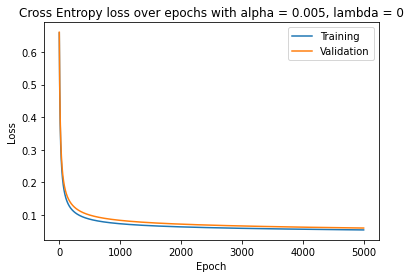
\includegraphics[scale=0.45]{images/loss reg 0 alp 005.png}}
  \hfill
  \subfloat{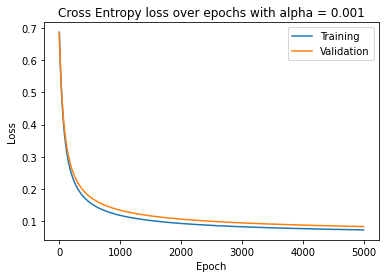
\includegraphics[scale=0.45]{images/loss reg 0 alp 001.png}}
  \hfill
  \subfloat{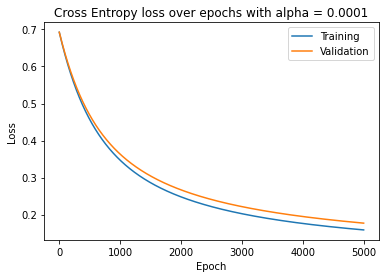
\includegraphics[scale=0.45]{images/loss reg 0 alp 0001.png}}
  \hfill
  \subfloat{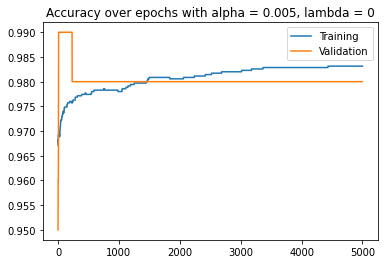
\includegraphics[scale=0.45]{images/acc reg 0 alp 005.png}}
  \hfill
  \subfloat{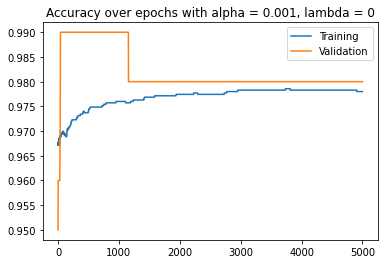
\includegraphics[scale=0.45]{images/acc reg 0 alp 001.png}}
  \hfill
  \subfloat{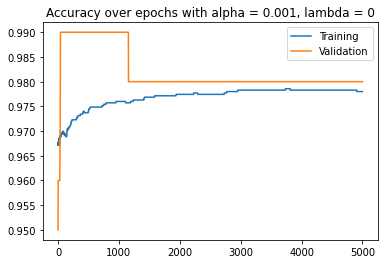
\includegraphics[scale=0.45]{images/acc reg 0 alp 0001.png}}
  \caption{Accuracy and loss graphs for training and validation data sets with varying
    alpha values}
\end{figure}

\subsection{Generalization}
The graphs shown below show the accuracy and loss of training and validation data with $\lambda = \{0.5, 0.1, 0.001\}$.
The hyperparameter $\lambda$ regulates how much of the euclidean norm of the weight vector needs to be added to the loss:
\begin{center}
  $\frac{\lambda}{2} ||\mathbf{w}||_2^2$
\end{center}
The main point of a regularization parameter is to make sure that the model doesn't get over-fit to the training data.
So the goal of this experiment was to find a suitable value for $\lambda$ that made sure the model wasn't over-fit.
However, one draw back of using a regularization factor is that it adds bias to the model.
In any case for this case a high $\lambda$ values makes the loss and accuracy converge quicker. However, the accuracy graphs
for $\lambda = 0.005$ and $\lambda = 0.001$ exhibited under-fitting and over-fitting respectively. Because of this, the best value
is $\lambda = 0.1$ because it converges quickly, taking only around 2000 epochs, has high accuracy (98\%) and low loss (0.11).

\begin{figure}[h]
  \subfloat{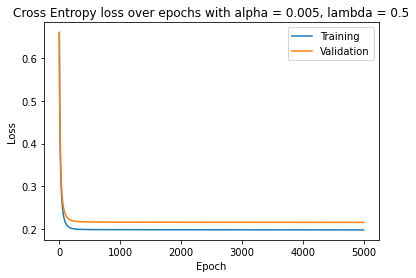
\includegraphics[scale=0.45]{images/loss reg 05 alp 005.png}}
  \hfill
  \subfloat{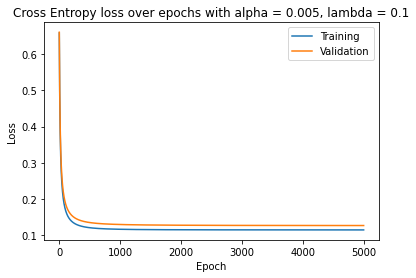
\includegraphics[scale=0.45]{images/loss reg 01 alp 005.png}}
  \hfill
  \subfloat{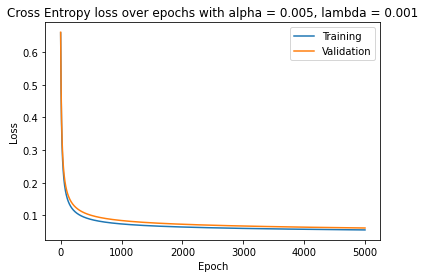
\includegraphics[scale=0.45]{images/loss reg 001 alp 005.png}}
\end{figure}

\begin{figure}[!tbp]
  \subfloat{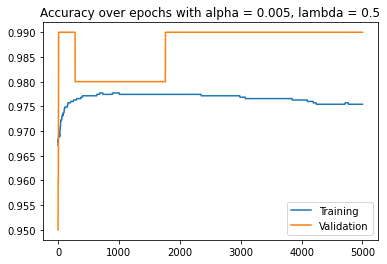
\includegraphics[scale=0.45]{images/acc reg 05 alp 005.png}}
  \hfill
  \subfloat{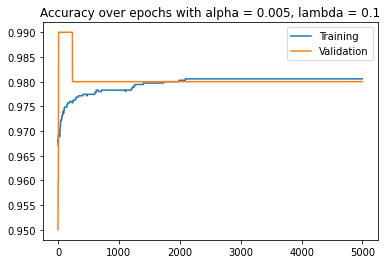
\includegraphics[scale=0.45]{images/acc reg 01 alp 005.png}}
  \hfill
  \subfloat{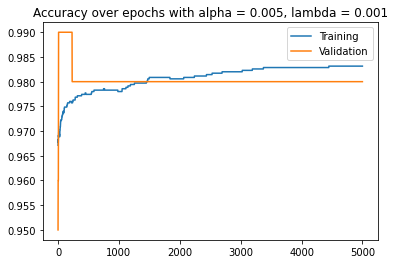
\includegraphics[scale=0.45]{images/acc reg 001 alp 005.png}}
  \caption{Loss and accuracy graphs with varying amounts of regularization}
\end{figure}

\section{Logistic Regression in TensorFlow}
\subsection{Building the Computational Graph}
Shown below is the code used to generate the graph for implementing gradient descent in TensorFlow.
One thing to note is that this is TensorFlow 1.15, and in the future using pyTorch is far easier.

\begin{minted}{python}
def buildGraph(bias=0, reg=0, b1=0.9, b2=0.999, eps=1e-08):

  # Make the weight and bias TF variables
  W = tf.Variable(tf.truncated_normal(shape=(1, 784), stddev=0.5, 
    dtype=tf.float32), name="weights", dtype=tf.float32)
  b = tf.Variable(bias, name="bias", dtype=tf.float32)

  # Data, labels, and lambda 
  data = tf.placeholder(tf.float32, (None, 784), name="data")
  labels = tf.placeholder(tf.float32, (None, 1), name="labels")
  lmbda = tf.constant(reg, tf.float32, name="lambda")

  valid_data = tf.placeholder(tf.float32, (None, 784), 
    name="validdata")
  valid_label = tf.placeholder(tf.float32, (None, 1), 
    name="validlabels")

  # y_hat = XWT (None, 784)()
  y_hat = tf.matmul(data, tf.transpose(W)) + b

  # Regularization term 
  regularization = (lmbda / 2.0) * tf.matmul(W, tf.transpose(W))

  # Loss tensor: cross entropy loss of X and the regularization term.
  # Sigmoid corss entropy will return a vector so to make it a 
  # single element add up all the elements using tf.reduce_sum
  ce_loss = tf.reduce_sum(tf.losses.sigmoid_cross_entropy(
    multi_class_labels=labels, logits=y_hat))
  ce_loss += regularization

  # Adam optimizer, and tell it to minimize our loss function
  optim = tf.train.AdamOptimizer(learning_rate=0.001, 
    beta1=b1, beta2=b2, epsilon=eps)
  optim = optim.minimize(loss=ce_loss)

  # Also calculate the validation loss 
  valid_y_hat = tf.matmul(valid_data, tf.transpose(W)) + b
  valid_ce_loss = tf.reduce_sum(tf.losses.sigmoid_cross_entropy(
    multi_class_labels=valid_label, logits=valid_y_hat))
  valid_ce_loss += regularization

  return W, b, data, y_hat, labels, ce_loss, optim, regularization, 
    valid_ce_loss, valid_data, valid_label
\end{minted}

\subsection{Implementing Stochastic Gradient Descent}
Shown below is the code that implements stochastic gradient descent. One problem that arose
is that it takes quite a while for the training to take place. This might be because of all of the
error calculations that hog the CPU.

\begin{minted}{python}
def train_model(X, Y, epochs, batch_size, learning_rate, bias=0, 
  reg=0, b1=0.9, b2=0.999, eps=1e-08):

  tf.reset_default_graph()
  train_ERROR = []
  train_ACCURACY = []
  valid_ERROR = []
  valid_ACCURACY = []

  # Get the place holders, etc... for the weights, bias...
  W, b, data, y_hat, labels, ce_loss, optim, reg, valid_ce_loss, 
    valid_data, valid_label = buildGraph(bias, reg, b1, b2, eps)
  
  # Create a node to initialize all varibles of the graph
  init_op = tf.global_variables_initializer()

  # Set a random uniform seed 
  tf.set_random_seed(1000)

  # Format the input data into a 1D vector, new shape should be:
  # (3500, 28, 28) -> (3500, 784)
  # So each row now corresponds to an image
  X_processed = tf.reshape(X, (X.shape[0], -1))
  processed_validData = tf.reshape(validData, (validData.shape[0], -1))

  with tf.Session() as sess:
    sess.run(init_op)
    print("Starting training...")
    print("Parameters (batch size, learning rate, samples) (", 
      batch_size, learning_rate, X.shape[0], ")")

    data_shuffled = X_processed.eval(session=sess)
    label_shuffled = Y
    evaled_validL = validTarget
    evaled_validD = processed_validData.eval(session=sess)

    for itteration in range(epochs):

      # Total number of batches is number of instances over batch size
      total_batches = int(X.shape[0] / batch_size)

      # Generate 3500 random indices so that we can reconstruct X, and Y
      # in a random order, while still maintaing the X -> Y relation 
      random_indices = np.random.permutation(int(X.shape[0]))

      data_batch = data_shuffled[random_indices]
      label_batch = label_shuffled[random_indices]

      batch_step = 0

      for items in range(total_batches):
        
        # On each iteration get a sample of batch_size images and 
        # there associated  Label
        data_batch_np = data_batch[batch_step:(batch_step + batch_size):]

        label_batch_np = label_batch[batch_step:(batch_step + batch_size):]

        # Create a feed dictionary to give tensorflow varibles that  
        # will be fed into place holders...
        feed = {
          data : data_batch_np,
          labels : label_batch_np,
          valid_label : evaled_validL,
          valid_data :  evaled_validD
        }

        # Run the optimizer 
        ret_optim, ret_W, ret_b, ret_err, ret_yhat, ret_reg, 
        ret_valid_ce_loss = 
          sess.run([optim, W, b, ce_loss, y_hat, reg, valid_ce_loss],
          feed_dict=feed)

        batch_step += batch_size
    
      # Calculate the loss and accuracy...
      # Use the returned predictions y_hat and compare them 
      # to the labelsConvert sign(ret_yhat) 
      # (which is either -1, 0, or 1) to 0 or 1
      predictions = tf.sign(tf.sign(ret_yhat) + 1)
      predictions = tf.cast(predictions, dtype=tf.dtypes.float32)

      results = tf.equal(predictions, tf.cast(label_batch_np, 
        dtype=tf.dtypes.float32))
      results = tf.cast(results, dtype=tf.dtypes.float32)

      accuracy = tf.math.reduce_mean(results).eval(session=sess)
      error = ret_err[0][0]

      train_ERROR.append(error)
      train_ACCURACY.append(accuracy)

      # Use the returned bias and weights to make a prediction 
      # on the validation data, them calculate 
      # the error and the accuracy
      validation_predictions = tf.matmul(tf.cast(processed_validData,
       dtype=tf.dtypes.float32), tf.transpose(ret_W)) + ret_b
      validation_predictions = tf.sign(tf.sign(validation_predictions) + 1)

      validation_results = tf.equal(validation_predictions, 
        tf.cast(validTarget, dtype=tf.dtypes.float32))
      validation_results = tf.cast(validation_results, dtype=tf.dtypes.float32)
      validation_results = tf.math.reduce_mean(validation_results)
        .eval(session=sess)

      valid_ACCURACY.append(validation_results)
      valid_ERROR.append(ret_valid_ce_loss[0][0])

    return train_ERROR, train_ACCURACY, valid_ERROR, valid_ACCURACY  
\end{minted}

\subsection{Batch Size Investigation}
Batch size has two impacts, firstly a larger batch size will result in a more stable learning process, this
is because more samples are used in the gradient descent and so will have a more uniform weighting. Furthermore,
using a larger batch size results in a far faster training time. Consider the first accuracy graph with a batch
size of 100, the training curve is erratic and irregular. Compare this curve to the training curve with a batch size of
1750 and it become evident of the stability that large batch sizes create. However, one down side to
using a larger batch size if that the rate at which the model converges towards a target accuracy is slower.

\begin{center}
  \begin{tabular}{||c c||}
    \hline
    Batch size & Convergence epoch \\
    \hline\hline
    100        & 100               \\
    \hline
    700        & 400               \\
    \hline
    1750       & 700               \\
    \hline
  \end{tabular}
\end{center}

All three batch sizes tested still hit around the same training accuracy. However, the models with larger batch sizes
were able to have sustained validation accuracy after there convergence point. The model using a batch size of 100 had
issues with maintaining the validation accuracy at the same level as the training accuracy. Due to this and the sheer
amount of time wasted, using a small batch size is ill advised. From this investigation it is fairly safe to say that
using a batch size of 700 is the best in terms of stability, rate of convergence, and time.

\begin{figure}[h]
  \centering
  \subfloat{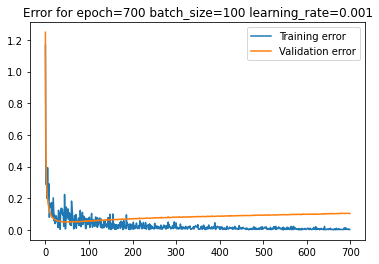
\includegraphics[scale=0.45]{images/loss epo 700 bs 100 lr 001.png}}
  \hfill
  \subfloat{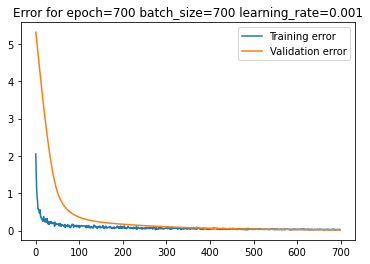
\includegraphics[scale=0.45]{images/loss epo 700 bs 700 lr 001.png}}
  \hfill
  \subfloat{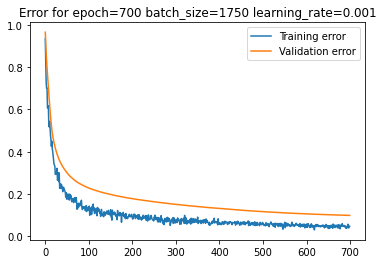
\includegraphics[scale=0.45]{images/loss epo 700 bs 1750 lr 001.png}}
  \hfill
  \subfloat{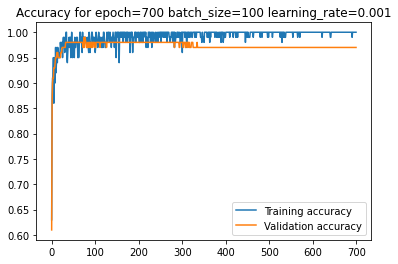
\includegraphics[scale=0.45]{images/acc epo 700 bs 100 lr 001.png}}
  \hfill
  \subfloat{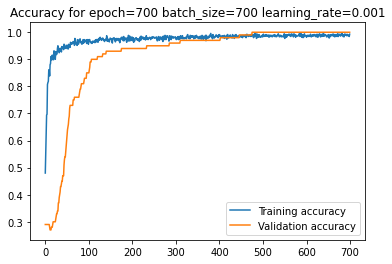
\includegraphics[scale=0.45]{images/acc epo 700 bs 700 lr 001.png}}
  \hfill
  \subfloat{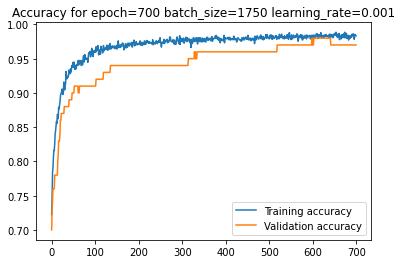
\includegraphics[scale=0.45]{images/acc epo 700 bs 1750 lr 001.png}}
  \caption{Loss and accuracy graphs with varying batch sizes}
\end{figure}

\newpage
\subsection{Hyperparameter investigation}

From this investigation a $\beta_1$ value of 0.95 is just slightly better because it offers a 97.9\%
accuracy on the testing data set. The best $\beta_2$ value is 0.99, firstly it achieved a 100\% accuracy
on the training data, but achieved 97.9\% on testing accuracy. The best $\epsilon$ value was difficult to choose,
they both perform equally on training, and validation accuracies. However, based on testing accuracy a value of $1*10^{-9}$
had a marginally better score at 97.9\%. 
\newline
Shown below is the accuracy and loss graphs for varying ADAM hyperparameters on the training, validation, and testing
data sets. Furthermore, the accuracy and loss are summarized in the following table:

\begin{center}
  \begin{table}[h]
    \centering
    \begin{tabular}{||c c c c c||}
      \hline
      Parameter  & Value  & Train & Validation & Test       \\
      \hline\hline
      $\beta_1$  & 0.95   & 0.992 & 0.96       & 0.97931033 \\
      $\beta_1$  & 0.99   & 0.982 & 0.96       & 0.9724138  \\
      \hline

      \hline
      $\beta_2$  & 0.99   & 1.0   & 0.98       & 0.97931033 \\
      $\beta_2$  & 0.9999 & 0.992 & 0.97       & 0.9724138  \\
      \hline

      \hline
      $\epsilon$ & 1e-09  & 0.994 & 0.98       & 0.97931033 \\
      $\epsilon$ & 1e-04  & 0.994 & 0.98       & 0.9724138  \\
      \hline
    \end{tabular}
    \caption{\label{tab: table-name}Comparing training, validation, and testing accuracies across different hyperparameters for ADAM}
  \end{table}
\end{center}

\begin{figure}[!]
  \centering
  \subfloat{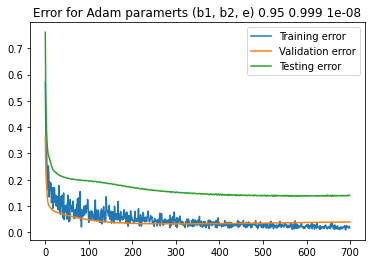
\includegraphics[scale=0.50]{images/loss b1 095.png}}
  \hfill
  \subfloat{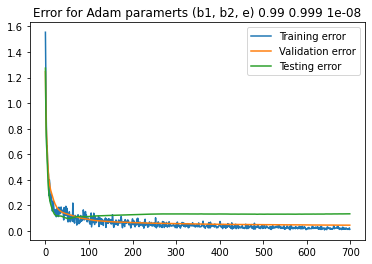
\includegraphics[scale=0.50]{images/loss b1 099.png}}
  \hfill
  \subfloat{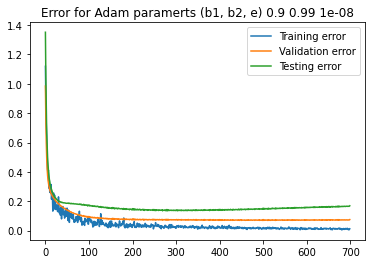
\includegraphics[scale=0.50]{images/loss b2 099.png}}
  \hfill
  \subfloat{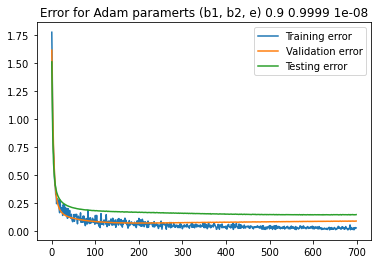
\includegraphics[scale=0.50]{images/loss b2 09999.png}}
  \hfill
  \subfloat{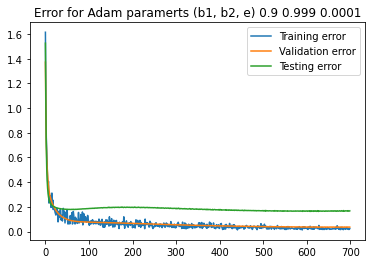
\includegraphics[scale=0.50]{images/loss e 0001.png}}
  \hfill
  \subfloat{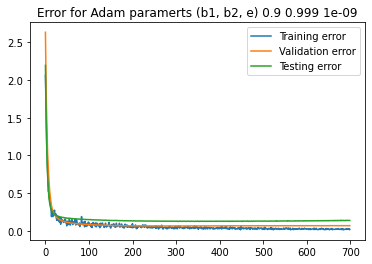
\includegraphics[scale=0.50]{images/loss e 1e-9.png}}
  \caption{Loss graphs with ADAM hyperparameters}
\end{figure}

\begin{figure}[!]
  \centering
  \subfloat{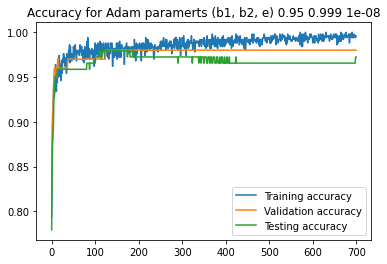
\includegraphics[scale=0.50]{images/acc b1 095.png}}
  \hfill
  \subfloat{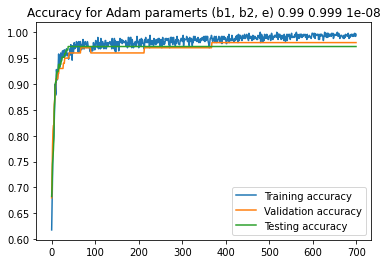
\includegraphics[scale=0.50]{images/acc b1 099.png}}
  \hfill
  \subfloat{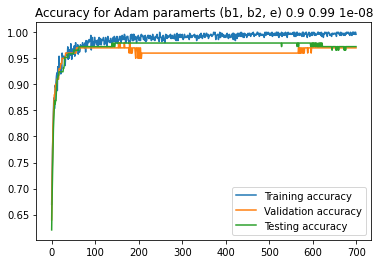
\includegraphics[scale=0.50]{images/acc b2 099.png}}
  \hfill
  \subfloat{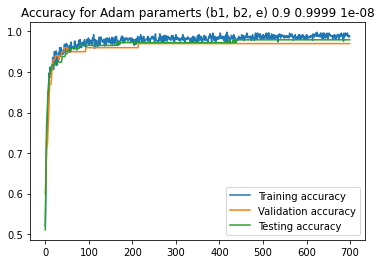
\includegraphics[scale=0.50]{images/acc b2 0999.png}}
  \hfill
  \subfloat{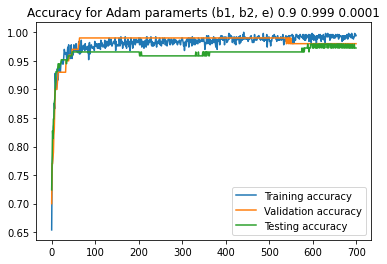
\includegraphics[scale=0.50]{images/acc e 0001.png}}
  \hfill
  \subfloat{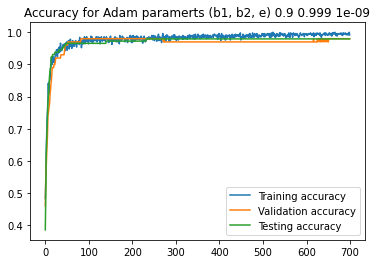
\includegraphics[scale=0.50]{images/acc e 1e-9.png}}
  \caption{Accuracy graphs with ADAM hyperparameters}
\end{figure}


\newpage
\subsection{Comparison against Batch GD}
All three methods were able to achieve similar accuracies, all reaching from 96\% to upwards of 99\%.
However, the rate at which the training accuracies, validation accuracies, and testing accuracies converged,
was vastly different across the two methods. SGD with ADAM was able to converge from as soon as 50 epochs,
to as late as 700 epochs. Compare this to batch GD which would converge starting at 1250 epochs to as late as
3000 epochs. So, in terms of efficiency SGD with ADAM is far superior, instead of spending time tuning the
model over thousands of epochs it could be better spent tuning hyperparameters. It's also important to note that
the loss for models using SGD with ADAM were generally lower than those using batch gradient descent.
The main defining trait that make SGD with ADAM better is the ability to tune hyperparameters. In the first
section the only parameters that could be adjusted were the batch size, training time, and learning rate. Whereas,
ADAM allows for much more fine tuned control, this combined with the quicker training times means that
more effort can be spent on extracting every bit of performance from the model, ie adjusting hyperparameters.
In the end SGD with ADAM offers more control, better performance, and more flexibility. Theses factors combined with 
the generally lower loss, higher accuracy (marginally), and faster rate of accuracy convergence makes it the far 
better model to use for future applications. 
\end{document}